\documentclass[letterpaper, 12pt]{article}


%\usepackage[lmargin=0.6in, rmargin=0.6in,tmargin=0.6in,bmargin=0.6in]{geometry}
%\pagestyle {empty}
%

\usepackage{amsmath,amssymb,amstext} % Lots of math symbols and environments
\usepackage{graphicx} % For including graphics N.B. pdftex graphics driver 

\begin{document}
%\chapter{Availability analysis of large and complex systems}
\title{Substation Reliability and Cost Analysis }
\author{Arun Veeramany and Mahesh D. Pandey \\
Department of Civil and Environmental Engineering, \\ University of Waterloo,
Waterloo, Ontario, N2L 3G1, Canada \\
aveerama@uwaterloo.ca }
\maketitle


\begin{abstract}
%% Text of abstract
A reliability model to study the effect of number of spares on a system comprising of a series of transformers in a substation is developed. 
%The model takes aging of the transformers in to consideration. 
This is achieved by developing a semi-Markov model assuming Weibull distribution for failure times. Further, it is assumed that the transformers are repairable. The results for both Markov and semi-Markov models are compared and the advantage of considering variability in failure times is demonstrated. Further, a substation cost model is developed to determine the ideal number of spares to have in the inventory.
\end{abstract}

{\bf \text{Keywords }\text{ }} spares, reliability, semi-Markov

%\begin{figure}[ht!] \centering
%  \includegraphics[scale=1.6]{ugf/TailGas/TailGasSchematic}
%  \caption{Schematic diagram of tail-gas quench and clean-up system\cite{Caceres1976} \label{fig:BridgeNetwork}} 
%\end{figure}


\section{Introduction}

Redundancies and spares are expensive, yet well established ways of preventing a mission critical system from failing. 
\cite{Silva2010} proposed Markov and Monte Carlo simulation methods to determine the optimal number of spares that minimize the total cost. The paper compared the obtained results against a model based on Poisson distribution. 
\cite{Marseguerra2005325} applied a combination of Monte Carlo simulation and genetic algorithms to optimize the number of spare parts required by a multi-component system. The objective was to maximize the system revenues and minimize the total spares volume. While the Markov model assumes constant failure rates irrespective of the variability in the transformer failure times, the Monte Carlo simulation is prone to large variability in reliability estimates and demands specialized variance reduction techniques. Hence, the present paper studies the effect of  number of spares on substation reliability based on the semi-Markov framework so that non-exponential distributions like Weibull can be considered in the model implementation. 
%The major advantage of this extension is to study the aging effects on the system. 
The paper further focuses on a predictive financial model to determine the ideal number of spares to invest upon in order to avoid economic losses due to unforeseen outages. The proposed model is of interest to technical personnel to have reliability estimates at hand and for station owners to decide how much investment needs to be made on spare transformers.



The paper is organized as follows. Section \ref{sec:SparesMarkovModel} discusses a Markov model for substation reliability. A subsection in it shows an example with two spares and develops the required differential equations.  The theory for semi-Markov model is covered in Section \ref{sec:SMPModel}. Section \ref{sec:SMPSpares} deals with the semi-Markov solution of the transformer problem. Markov and semi-Markov results are shown for a 12 transformer system with different number of spares. 
The Markov reward (cost) model is reviewed in Section \ref{sec:MarkovRewardModel}. Section \ref{sec:SparesMarkovRewardModel} develops the cost model for determining losses due to repairs and outages. Results are reported in Section \ref{sec:SparesResults}. 


\section{Markov model}
\label{sec:SparesMarkovModel}

\begin{figure}[h!] \centering
  \includegraphics[scale=0.9]{SparesStateSpace}
  \caption{State space for $N$ Transformers with $n$ Spares.\label{fig:SparesStateSpace}} 
\end{figure}

Consider $N$ transformers connected in series with $n$ spares available for replacement on failure of any of the operational transformers. It is assumed that when all the spares are used up and at least one of the transformers in use fails, then the system fails. Further, the time taken to replace a failed transformer with a spare is assumed to be negligible. While a single transformer could fail with a failure rate of $\lambda$, it can be repaired with a repair rate of $\mu$. The state space diagram for this model is shown in Figure \ref{fig:SparesStateSpace}. For a system with $n$ available spares there are $n+2$ states in the model. Assume that the system starts in state $n+1$ where all the transformers are functional and all  the spares are readily available. Then, the probability of landing in state 0 gives the failure probability of the system.
The model in \cite{Silva2010} assumes that two or more transformers are connected in parallel. In the present paper, the same model is considered without redundancies.

\subsection{Example: 12 Transformers and 2 Spares}
\label{sec:TwoSparesExample}
\begin{figure}[h!] \centering
  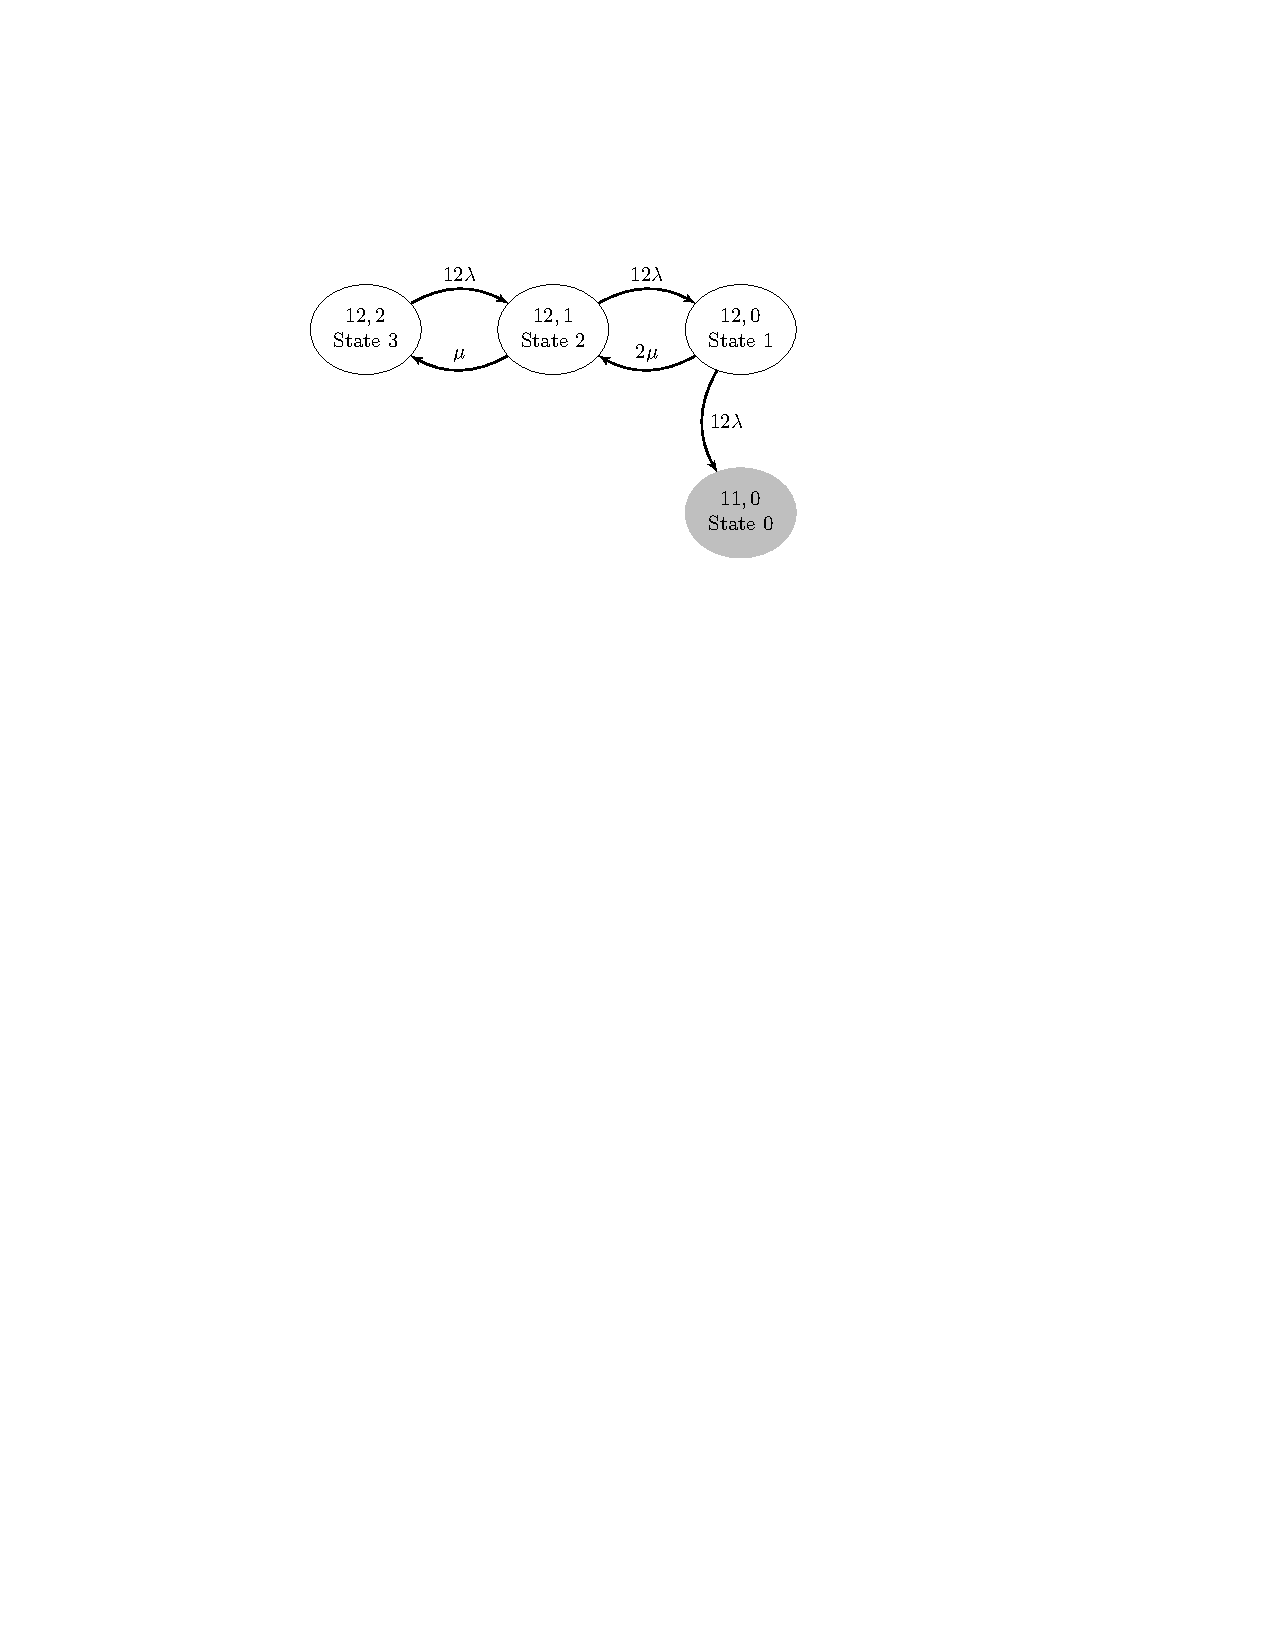
\includegraphics[scale=0.9]{TwoSparesStateSpace}
  \caption{State space for $N=12$ Transformers with $n=2$ Spares.\label{fig:TwoSparesStateSpace}} 
\end{figure}
In particular, consider an example with $N=12$ transformers and $n=2$ spares. The Markov transition rate matrix for this case is given by:
\begin{align}
A=
\begin{bmatrix}
0	 & 	0	 & 	0	 & 	 0	\\
N\lambda	 & 	-( N\lambda + 2\mu)	 & 	2\mu	 & 	0	\\
0	 & 	N\lambda	 & 	-( N\lambda + \mu)	 & 	\mu	\\
0	 & 	0	 & 	N\lambda	 & 	-N\lambda 
\end{bmatrix}
\end{align}

Let $\mathbf{P}(t)$ be a row vector of state probabilities to be determined:
\begin{align}
\mathbf{P}(t) = [p_0(t) \text{ } p_1(t) \text{ } p_2(t) \text{ } p_3(t)]
\end{align}

Then, the system of differential equations to obtain the state probabilities can be compactly written in matrix form:
\begin{align}
\frac{d\mathbf{P}(t)}{dt} = \mathbf{P}(t) A
\end{align}
or elaborately as:
\begin{align}
dp_0(t)/dt &=N\lambda p_1(t)	\nonumber \\
dp_1(t)/dt &=N\lambda p_2(t) -( N\lambda + 2\mu)p_1(t)	\nonumber \\
dp_2(t)/dt &=2 \mu p_1(t) +N\lambda p_3(t) -( N\lambda + \mu)p_2(t)	\nonumber \\
dp_3(t)/dt &= \mu p_2(t) -N\lambda p_3(t) \nonumber \\
\end{align}

$p_0(t)$ yields the failure probability of the system assuming the initial state vector as [0 0 0 1].


\section{The Semi-Markov Process Model}
\label{sec:SMPModel}
This project follows the general formulation of the continuous-time discrete-state semi-Markov process model as developed in \cite{HowardA} and \cite{HowardB}. 

Let the model have $N$ states. Let $f_{ij}(t)$ and $F_{ij}(t)$ represent the   $pdf$ and $cdf$ respectively of the event corresponding to the transition from state $i$ to state $j$ at time $t$. 

Assume that the process is in state $i$. From this state, there could be $k$ different states to which the process could transit to in a single step. Also assumed in this model is that all these $k$ possibilities are independent of the occurrence of each other. At a time instant $t$, the process chooses only one state from these choices such that the time to be spent in the current state $i$ is the minimum before instantaneously jumping to the chosen state. The probability that the next state is $j$ and not any other state $k$ reachable from $i$ is given by:
\begin{align}
\label{eq:CompRisk}
c_{ij}(t) =  f_{ij} (t)\prod\limits_{k \ne j} {(1 - F_{ik} (t))} 
\end{align}
For $N$=2, $c_{ij}(t) =  f_{ij} (t)$. The matrix $C(t)=[ c_{ij}(t) ]$ is called the kernel or core of the semi-Markov process model and
\begin{align}
\label{eq:waiting}
w_i(t) = \sum\limits_{j=1}^{N}{c_{ij}(t)}
\end{align}
is called the waiting time distribution for the state $i$. It represents the probability that the process waits in state $i$ for $t$ time units before making a transition. Hence it is an unconditional probability distribution. 
It is assumed that any row $i$ of the kernel $C=[c_{ij}]$ satisfies the condition:
\begin{eqnarray}
\int\limits_0^\infty  { \sum\limits_{j}^{}{c_{ij}(t)} dt \approx 1} 
\label{eq:MREAssumption}
\end{eqnarray}
This assumption assures that there is unit probability that the process
will be in one of the $N$ states of the process at time $t$, given the initial 
state as $i$. The probability that the process does not leave state $i$ by time $t$ is given by:
\begin{align}
\label{eq:staying}
W_i (t) = 1 - \int\limits_0^t {w_i(t)dt} 
\end{align}
The objective of the model is to determine the probability $\phi_{ij}(t)$  of being in each state  $j$ given that the process initially is in a particular state $i$. $\phi_{ij}(t)$  can be determined by solving a system of integral equations:
\begin{align}
{\phi _{ij} (t)} = \delta _{ij} W_i (t) + \sum\limits_k {\int\limits_0^t {c_{ik} (\tau ){\phi _{kj} (t - \tau )}d\tau } } 
\label{CTMRE}
\end{align}
Where $i=j=k=0,1,2,...N-1$.	 


The right hand side of Equation \ref{CTMRE} describes the following probabilities:
\begin{enumerate}
\item	$i=j$ and second term=0: $W_i (t)$ is the probability that the process does not leave state $i$ by time $t$.
\item	$i=j$ and second term not 0: process leaves state $i$ and returns to $i$ by time $t$.
\item	$i \neq j$  and second term $\neq j$ : process leaves state $i$ and reaches state $j$ by time $t$.
\end{enumerate}
The system of equations can alternatively be written in a compact form as a matrix:
\begin{align}
{\phi(t)} = diag(W(t)) + {\int\limits_0^t {C(\tau ){\phi (t - \tau )}d\tau } } 
\label{MatMRE}
\end{align}






\section{Semi-Markov model for substation reliability}
\label{sec:SMPSpares}
The kernel matrix of the semi-Markov process model consists of statistical distributions respecting the competing risk law of Equation \ref{eq:CompRisk} instead of constant transition rates. The failure time distributions are modeled as poly-Weibull distributions while the repair times follow an exponential distribution. This section describes how these distributions can be used to construct the kernel matrix.

The $cdf$ of the poly-Weibull distribution for the transition time corresponding to the failure rate $N\lambda$ in the Markov model of Figure \ref{fig:SparesStateSpace} is given by:
\begin{align}
F_{i, i-1}(t) = 1 - e^{-N(\lambda^{'} t)^{\gamma}}
\label{eqn:PolyWblSparesCDF}
\end{align}
where the subscript ${i, i-1}$ represents the transition from state $i$ to $i-1$ signifying failure of a transformer and replacement by a spare.

The corresponding $pdf$ is found by differentiating Equation \ref{eqn:PolyWblSparesCDF}:
\begin{align}
f_{i, i-1}(t) = N(\lambda^{'}\gamma) (\lambda^{'} t)^{\gamma-1}e^{-N(\lambda^{'} t)^{\gamma}}
\label{eqn:PolyWblSparesPDF}
\end{align}


Assuming that the repair time follows an exponential distribution, the $cdf$ of the time to repair is the minimum of all the times taken to repair the failed $k$ transformers each having a repair rate of $\mu$:
\begin{align}
G_{i, i+1}(t;k) = 1 - e^{-k\mu t} \hspace{1in} i\neq 0
\label{eqn:ExpSparesCDF}
\end{align}

The corresponding $pdf$ is:
\begin{align}
g_{i,i+1}(t;k) = k\mu e^{-k\mu t}	\hspace{1in} i\neq 0
\label{eqn:ExpSparesPDF}
\end{align}

The kernel matrix $C(\tau) = [c_{ij}(\tau)]$ is given by arranging the distribution functions as per Equation \ref{eq:CompRisk}:
\begin{align*}
\bordermatrix {
	&	0	&	1	&	2	&	.	&	n	&	n+1	\\
0	&	0	&	0	&	0	&	.	&	0	&	0	\\
1	&	f_{10}(\tau)[1-G_{12}(\tau;n)]	&	0	&	g_{12}(\tau;n)[1-F_{10}(\tau)]	&	.	&	0	&	0	\\
.	&	.	&	.	&	.	&	.	&	.	&	.	\\
.	&	.	&	.	&	.	&	.	&	.	&	.	\\
n+1	&	0	&	0	&	0	&		&	f_{n+1,n}(\tau)	&	0	\\
}
\end{align*}

The integral equations corresponding to the above kernel matrix can be formulated based on Equation \ref{CTMRE}. The system is then solved using numerical scheme like trapezoidal rule as given in the appendix. Assuming that the system starts functioning in state $n+1$, the probability of being in state 0 denoted by $\phi_{n+1,0}(t)$ gives the system failure probability.


The system of integral equations for $N=12$ and $n=2$ is given as an example in the appendix.


\begin{figure}[h!] \centering
  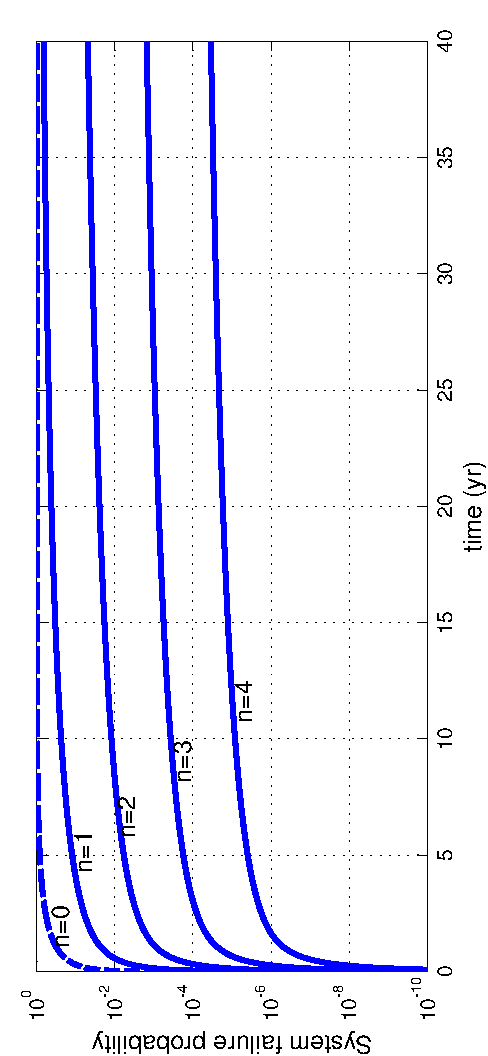
\includegraphics[scale=0.8, angle=-90]{ExpFailureProb}
  \caption{System failure probability with exponential failure and repair time; 12 transformers and $n=0,1,2,3,4$ spares.\label{fig:ExpFailureProb}} 
\end{figure}

Considering a constant failure rate of $\lambda=0.03$ per year and a repair rate of 4 per year for a transformer and supposing there are $N=12$ such transformers connected in series, Figure \ref{fig:ExpFailureProb} shows the system failure probability by solving the system of differential equations of the Markov model and the system of integral equations of the semi-Markov model proving that the results are identical no matter which method is used by assuming an exponential distribution for both failure and repair times. 
In both cases, varying number of spares were considered. It is also observed that failure probability is inversely related to the number of spares $i.e.$, system reliability improves with increased number of spares. 

\begin{figure}[h!] \centering
  \includegraphics[scale=0.8, angle=-90]{CompareWblExp}
  \caption{System failure probability comparing Webull and exponential failure time; 12 transformers and 2 spares.\label{fig:CompareWblExp}} 
\end{figure}

\begin{figure}[h!] \centering
  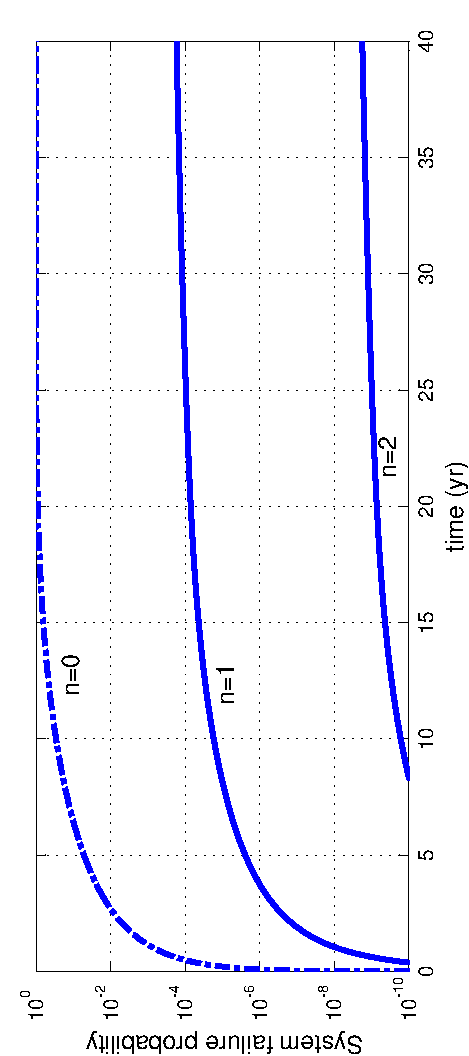
\includegraphics[scale=0.8, angle=-90]{WblFailureProb}
  \caption{System failure probability with Webull failure time and exponential repair time; 12 transformers and $n=0,1,2$ spares.\label{fig:WblFailureProb}} 
\end{figure}

In the absence of spares, system failure probability reaches 0.9999 at the end of 40 years. In this scenario, there are only two states in the system and either all the transformers are functional or the system fails due to failure of one of the transformers. Addition of a spare lowers the failure probability to $0.667$ thus boosting the system reliability by approximately $33\%$. In this case, there are three states in the system. When one of the spares is used, the failed transformer can undergo repair. After completion of the repair, a spare can be made available again. However, if one of the transformers fails when the spare is being used, then the system fails as the earlier failed transformer is still under repair. Adding further spares increase the reliability, however, beyond a certain number of spares, the system would become too reliable to afford the spares.


Figure \ref{fig:CompareWblExp} compares the system failure probability for the case of two spares assuming exponential and Weibull failure times respectively at the end of 40 years. A $cov$ of 0.4 is assumed for the Weibull case. While the system failure probability for the exponential case is 4.92 x $10^{-2}$, the same for Weibull case is 1.76 x $10^{-9}$ signifying that lower variability in failure times yields higher reliability. 
The same trend is observed for varying number of spares in Figure \ref{fig:WblFailureProb} assuming Weibull transformer failure times. Random failures often show up large variation in failure times whereas those of a cohort of aging transformers are likely to show less variability. 


\begin{table}[!h] \centering
\caption{System failure probability as a function of number of spares at $t=40$ years\label{tbl:SysRelImprovement}}
\begin{tabular}{c | r  r }
\hline
					& \multicolumn{2}{| c}{Failure time}\\
			&		\multicolumn{2}{|c}{-----------------------------------------------} \\
\# Spares	&	Exponential ($cov=1$)			&	Weibull ($cov=0.4$) \\
\hline					
0	&	0.9999	&	0.9999	\\
1	&	6.67 x $10^{-1}$	&	1.70 x $10^{-4}$	\\
2	&	4.92 x $10^{-2}$	&	1.76 x $10^{-9}$	\\
3	&	1.53 x $10^{-3}$	&	6.15 x $10^{-15}$	\\
4	&	3.47 x $10^{-5}$	&	9.89 x $10^{-21}$	\\
\hline					
\end{tabular}
\end{table}


Table \ref{tbl:SysRelImprovement} compares the effect of adding more spares to a system at the end of 40 years by assuming Weibull and exponential transformer failure times respectively. A $cov$ of 0.4 was assumed for the Weibull case.
In both cases, the repair time is exponentially distributed. Both the results show that the system performs better by having more spares. The failure probability when there are no spares is very high. Since it is assumed that the transformer failure time is less variable in the Weibull case, the system failure probability drops to 1.76 x $10^{-9}$ by having one spare against no spares. 
When system reliability is analyzed along with a financial model, these results can have a profound impact on decision making and budget allocation with respect to spare handling. However, one has to invest in more accurate and regular reporting of transformer failure times if variability is also needed as the input. In either case, simultaneous transformer failures due to common cause failures is not considered in the present paper. The next section explores the Markov reward model as an aid in deciding the ideal number of spares to have in the stock.

\section{Markov reward model}
\label{sec:MarkovRewardModel}
The Markov reward model was initially developed keeping cost and financial models in mind. An example in the case of a multi-state repairable component was cited by \cite{Lisnianski2003}. The continuous-time Markov chain and the Markov transition rate matrix form the basis for this model. Additionally, each state transition and stay in a state is associated with a reward. This reward can be positive when it fetches profit or negative when it signifies losses. For developing a cost model, reward can be the associated loss due to a failure or the cost incurred on a repair or profit due to a sale. These rewards are arranged in a separate matrix which is similar in dimension to the transition rate matrix. Given these as the input along with the initial conditions, the total expected reward accumulated up to time $t$ can be obtained:
\begin{align}
\frac{dV_i(t)}{dt} = r_{ii} + \sum_{j=1, j \neq i}^{K}{a_{ij}r_{ij}} + \sum_{j=1}^{K}{a_{ij}V_j(t)}
\label{eq:RewardEquationForm}
\end{align}
where,
\begin{itemize}
\item $V_i(t)$ is the total expected reward accumulated up to time $t$ with $i$ as the initial state  of the process at time 0,
\item $r_{ii}$ is the reward per unit time for staying in state $i$,
\item $r_{ij}$ is the reward for the transition from state $i$ to state $j$,
\item $a_{ij}$ is the $(i,j)th$ element of the transition rate matrix.
\end{itemize}

Equation \ref{eq:RewardEquationForm} can be written in a matrix form as:
\begin{align}
\frac{d}{dt} \pmb{V(t) = u + aV(t)}
\label{eq:RewardMatrixForm}
\end{align}
where,
\begin{align}
u_i = r_{ii} + \sum_{j=1, j \neq i}^{K}{a_{ij}r_{ij}} 
\label{eq:UInRewardEqn}
\end{align}

The above system can be solved with $V_i(0)=0$ for all $i$ as the initial condition. Once solved, $V_i(t)$ with $i$ as the initial state yields the required average reward accumulated up to time $t$.





\section{Cost Model for Substation Spares}
\label{sec:SparesMarkovRewardModel}
\begin{figure}[h!] \centering
  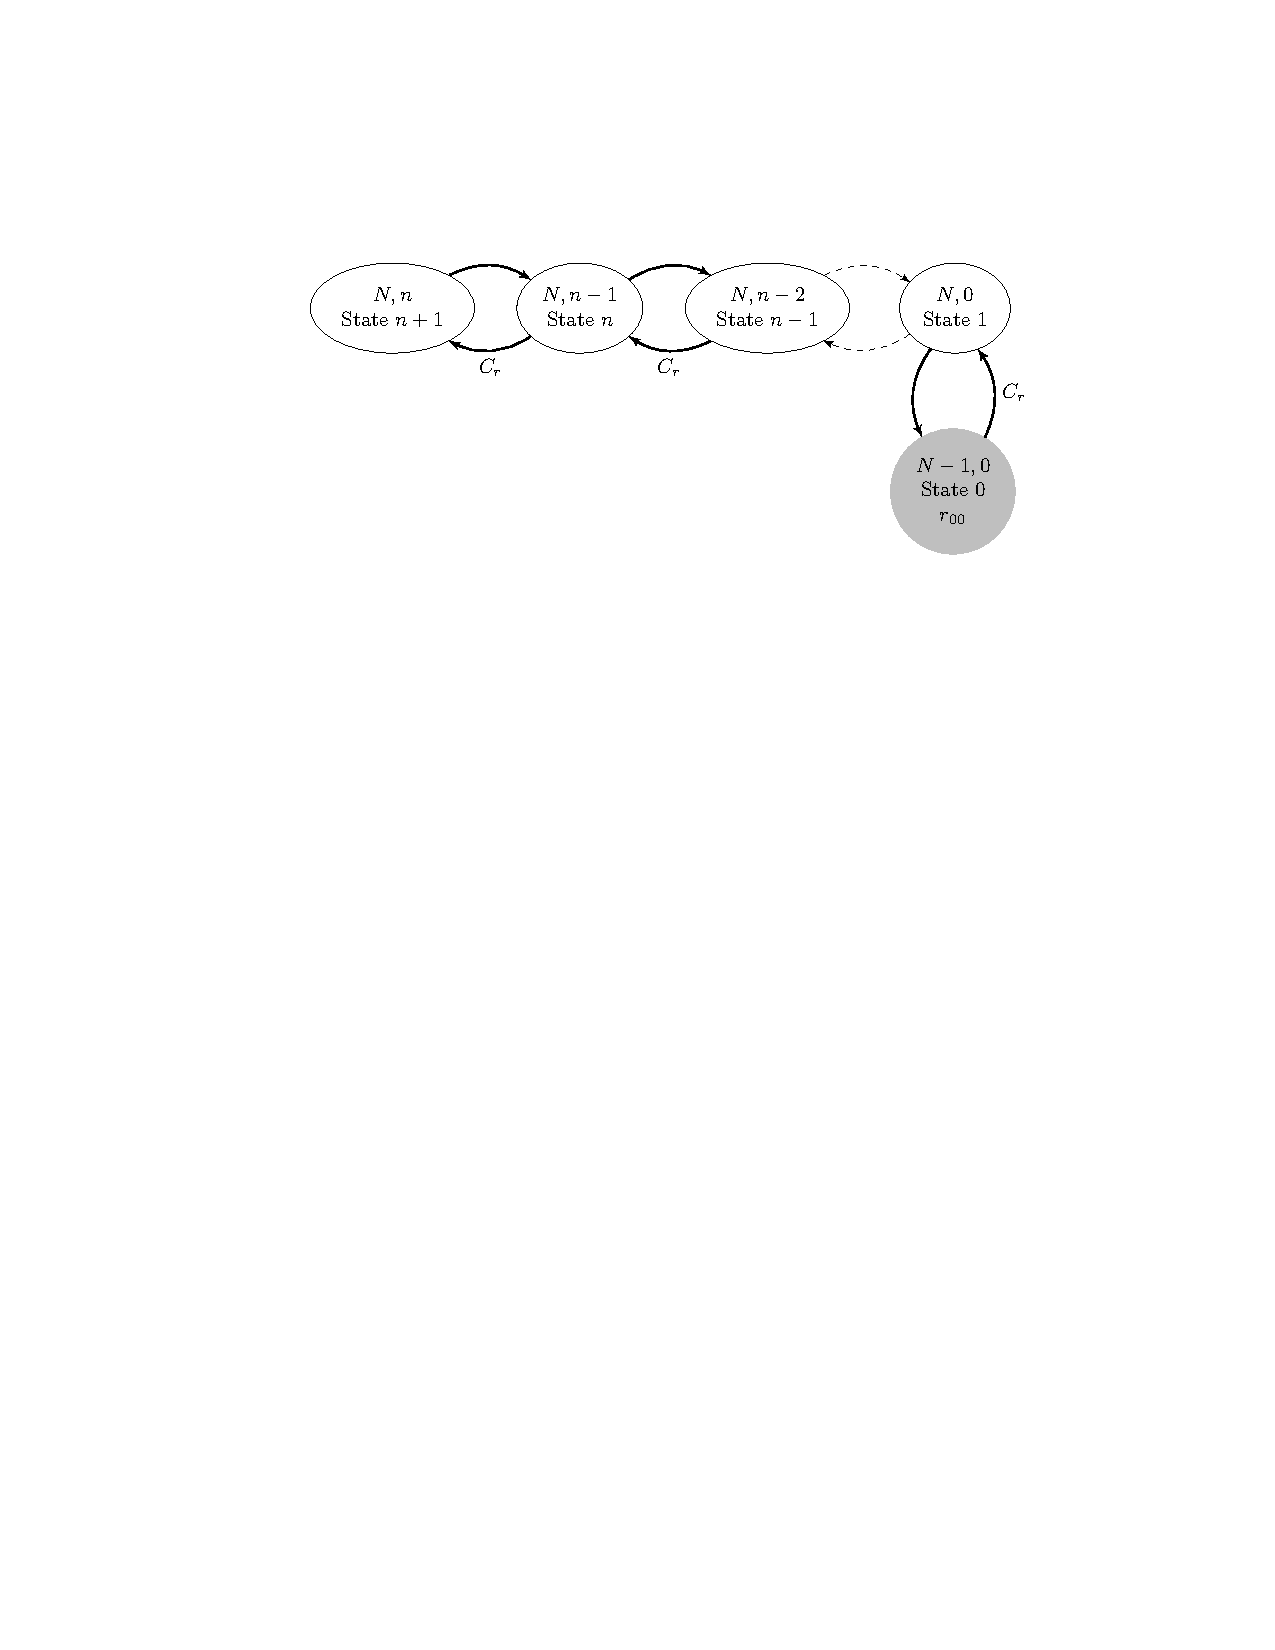
\includegraphics[scale=0.9]{RewardStateSpace}
  \caption{Markov Reward Model for $N$ Transformers with $n$ Spares.\label{fig:RewardStateSpace}} 
\end{figure}
The state space for the reward model is similar to the Markov model of Figure \ref{fig:SparesStateSpace} except that the system is assumed to be repairable from state 0. Each repair is assumed to cost $C_r$ million dollars. A loss of $r_{00}$ million dollars per year is assumed on an outage which is equivalent to the process staying in state 0 and waiting for a system repair to be completed. This loss is based on kilowatts of energy per year not supplied to the consumer until the system goes online again.


The Markov reward model with the specifications described is shown in Figure \ref{fig:RewardStateSpace}. The Markov reward matrix $r$ is a square matrix obtained from the state space:

\begin{align}
\bordermatrix{
		&		0					&		1			&		2			&		. . . & n+1 \cr
0 	& 	r_{00}		&		C_r		&		0			&		. . . & 0 \cr
1		&		0					&		0			&		C_r		&		. . .	&	0	\cr
. 	&		.					&					&					&					&		\cr		
. 	&							&		.			&					&					&		\cr
. 	&							&					&		.			&					&		\cr
n		&		0					&		0			&		0			&		. . . & C_r \cr
n+1	&		0					&		0			&		0			&		. . . & 0
}
\end{align}


\section{Results and discussion}
\label{sec:SparesResults}
\begin{table}[!h]\centering
\caption{Parameters for evaluating the cost model\label{tbl:SparesParamTable}}
\begin{tabular}{l l l}
\hline					
Symbol	&	Description	&	Assumed Value	\\
\hline					
$\lambda$	&	Failure rate of transformer	&	0.03 $yr^{-1}$	\\
$\mu$	&	Repair rate of transformer	&	4 $yr^{-1}$	\\
$N$	&	Number of transformers connected in series	&	12	\\
$n$	&	Number of required  spares	&	0,1,2,. . .	\\
$L$	&	Nominal capacity of one transformer	&	$10^{5}$ kW	\\
$C_r$	&	Expected cost of repair 	&	C\$ 0.05 million	\\
& of one transformer &  \\
$C_j$	&	Expected cost of one spare transformer	&	C\$ 8 million	\\
$C_p$	&	Cost of Energy Not Supplied (ENS) per kWh	&	C\$ 1.00	\\
$r_{00}$	&	Cost of ENS per year  = $C_p  L$ x 8760	&	 C\$ 876 million	\\
$m$	&	Assumed lifespan of a plant	&	40 years	\\
$r$	&	Discount rate	&	0.07	\\
\hline					
\end{tabular}
\end{table}

The list of symbols in the model and the assumed values are listed in Table \ref{tbl:SparesParamTable}.

\begin{figure}[h!] \centering
  \includegraphics[scale=0.8, angle=-90]{CumulativeRewards}
  \caption{Expected Cumulative Losses for 12 Transformers and $n$ Spares.\label{fig:CumulativeRewards}} 
\end{figure}


The accumulated economic loss due to repairs and outages up to $m$ years is shown in Figure \ref{fig:CumulativeRewards}. The reward model does not yet consider the investment on procuring the spares. It is seen that the expected loss is the maximum when there are no spares available in the inventory. For 1,2 or 3 spares, the expected loss decreases and then it is observed that the average loss is the same no matter how many more spares are added.

To get a complete picture, the amount invested on the spares and the net present cost obtained by combining the investment and the net present value of the expected losses is investigated in the next step.

From the cumulative expected losses $V_4(t)$ of the reward model, from hereon referred to as $V(t)$, the annual combined cost of repairs and outages can be calculated as $v_k=V(k+1) - V(k)$ for $k=1,2,3,..m$ for the $m$ years under consideration. The net present value of the losses is represented as $L_j$, where $j$ represents the number of spares. The NPV $L_j$ of the annual costs $v_1, v_2,..v_m$ discounted at a rate $r$ over $m$ years is then calculated as:
\begin{align}
L_j = \sum_{i=1}^m \frac{v_i}{(1+r)^i}
\end{align}
Let $C_j$ denote the investment made on procuring $j$ spares. The net present cost of losses and investments for $j$ spares is given by $A=L_j + C_{j}$. The objective then is to determine for what $j$ the value of $A$ is minimum.



\begin{table}[!h]\centering
\caption{Net present cost of investments and losses\label{tbl:SparesPresentCost}}
\begin{tabular}{l l l l}
\hline
Spares	&	Investment	&	NPV of Losses	&	Net Present Cost	\\
$j$	&	$C_j$	&	$L_j$	&	$C$ = $L_j+C_j$	\\
	& C\$ million & C\$ million & C\$ million \\
	\hline
0	&	0	&	949.01	&	949.01	\\
1	&	8	&	42.37	&	50.37	\\
2	&	16	&	1.49	&	17.49	\\
3	&	24	&	0.26	&	24.26	\\
4	&	32	&	0.24	&	32.24	\\
5	&	40	&	0.24	&	40.24	\\
\hline							
\end{tabular}
\end{table}						

Table \ref{tbl:SparesPresentCost} tabulates the net present cost as a function of number of spares. It is seen that the NPV of the losses remains constant beyond three spares. The net present cost is 949 million dollars in the absence of spares highlighting the huge risk involved in running a generating station without spares. With addition of two spares, the net present cost is seen to decrease to nearly 18 million dollars and then increases monotonically if the station decides to invest in more than two spares. This concludes that for the given configuration and assumed costs, it is optimal to have two spares always in the inventory.

\begin{figure}[h!] \centering
  \includegraphics[scale=0.8, angle=-90]{npv}
  \caption{Net present cost vs.the number of spares.\label{fig:npv}} 
\end{figure}

Figure \ref{fig:npv} shows graphically the trend seen in Table \ref{tbl:SparesPresentCost}. A simple and final plot as this is of great aid to decision makers for budget allocation and for the smooth and reliable running of the station.


\section{Conclusion}
A semi-Markov model with Weibull failure times was developed for assessing reliability of substation transformers. Results were compared against a Markov model and was proved that knowledge of variability in failure times of the transformers helps in obtaining more accurate estimates of system reliability. The Markov model was further extended to a Markov reward model to determine the number of spares to have in the inventory at all times to avoid economic losses due to unforeseen outages.



���}	� �
����DEV��INO��SYN��SV~�SparesAppendix.tex�NO�NP��NOq8�/P�_.q9


% The following statement selects the style to use for references.  It controls the sort order of the entries in the bibliography and also the formatting for the in-text labels.
\bibliographystyle{ieeetr}

% This specifies the location of the file containing the bibliographic information.  It assumes you're using BibTeX (if not, why not?).
\bibliography{uw-ethesis}
% Tip 5: You can create multiple .bib files to organize your references. 
% Just list them all in the \bibliogaphy command, separated by commas.
%\nocite{*}




\end{document}
